\section{Design Patterns}
    In software engineering, design patterns are common solutions for recurring problems encountered when building complex software. A design pattern can be described as a tried and tested blueprint based on well-known object-oriented principles, such as the SOLID\footnote{SOLID is an acronym that represents five important design principles for object-oriented programming. These are: Single Responsibility Principle, Open/Closed Principle, Liskov Substitution Principle, Interface Segregation Principle, and Dependency Inversion Principle. The purpose of these principles is to improve maintainability, readability, and extensibility.} principles that can be applied in many different contexts to solve various problems.

    Christopher Alexander initially introduced the idea of patterns in his book, "A Pattern Language: Towns, Buildings, Construction.". In this work, he presented a "vocabulary" for designing urban landscapes. The building blocks of this vocabulary consist of patterns that address various aspects of urban design, such as the height of windows, the number of floors in a structure, the size of green spaces within a community, and other similar elements.

    This concept was later adapted by the "Gang of Four" (Erich Gamma, Richard Helm, Ralph Johnson, and John Vlissides) and translated to the domain of software engineering in their seminal book "Design Patterns: Elements of Reusable Object-Oriented Software," which was published in 1994. This book offers a catalog of 23 reusable design patterns for object-oriented programming that are based on industry experience and observations from the authors.

    Today, many design patterns have been integrated into programming languages themselves and are therefore taken for granted by users. For example, the Visitor pattern (Figure \ref{fig:visitor-pattern-example}) is a behavioral design pattern that allows you to separate the algorithm from the object structure it is supposed to operate on. One concrete realization of the Visitor pattern's integration into a modern programming framework can be found in the ubiquitous for-each loop (Figure \ref{fig:for-loop-example}). The for-each loop allows for iteration over a collection of elements without the need for an explicit counter index, effectively separating the algorithm responsible for the iteration from the underlying data structure.

\begin{figure}[!ht]
    \begin{lstlisting}[style=csharp]
static void DoubleAndLog(int number)
{
    Console.WriteLine(number * 2);
}

List<int> numbers = new List<int> { 1, 2, 3, 4, 5 };
numbers.ForEach(DoubleAndLog);
    \end{lstlisting}
    \caption{For-each loop implementing Visitor pattern}
    \label{fig:visitor-pattern-example}
\end{figure}

\begin{figure}[!ht]
    \begin{lstlisting}[style=csharp]
List<int> numbers = new List<int> { 1, 2, 3, 4, 5 };

for (int i = 0; i < numbers.Count; i++)
{
    Console.WriteLine(numbers[i] * 2);
}
    \end{lstlisting}
    \caption{For-loop}
    \label{fig:for-loop-example}
\end{figure}

\subsection{The Observer Pattern}
One of the first design patterns introduced in the aforementioned book by the “Gang of Four”, the Observer pattern is a behavioral pattern that addresses several different key problems in object-oriented programming. It is implemented by creating two separate interfaces: the publisher who is responsible for publishing events of interest for the rest of the system, and subscribers who are interested in knowing when the publisher has published such an event. Implementing these interfaces allows the system to achieve loose coupling, as the publisher and subscribers can evolve independently, promoting a maintainable and adaptable system. Developers can easily introduce new subscribers with minimal modifications. Furthermore, the pattern facilitates dynamic relationships between scripts that can change at runtime by having the subscribers unsubscribe from the publisher. This, accompanied by the publisher's event broadcasting ability, ensures that the entire system remains in a consistent and traceable state. 

    \begin{figure}[H]
      \centering
      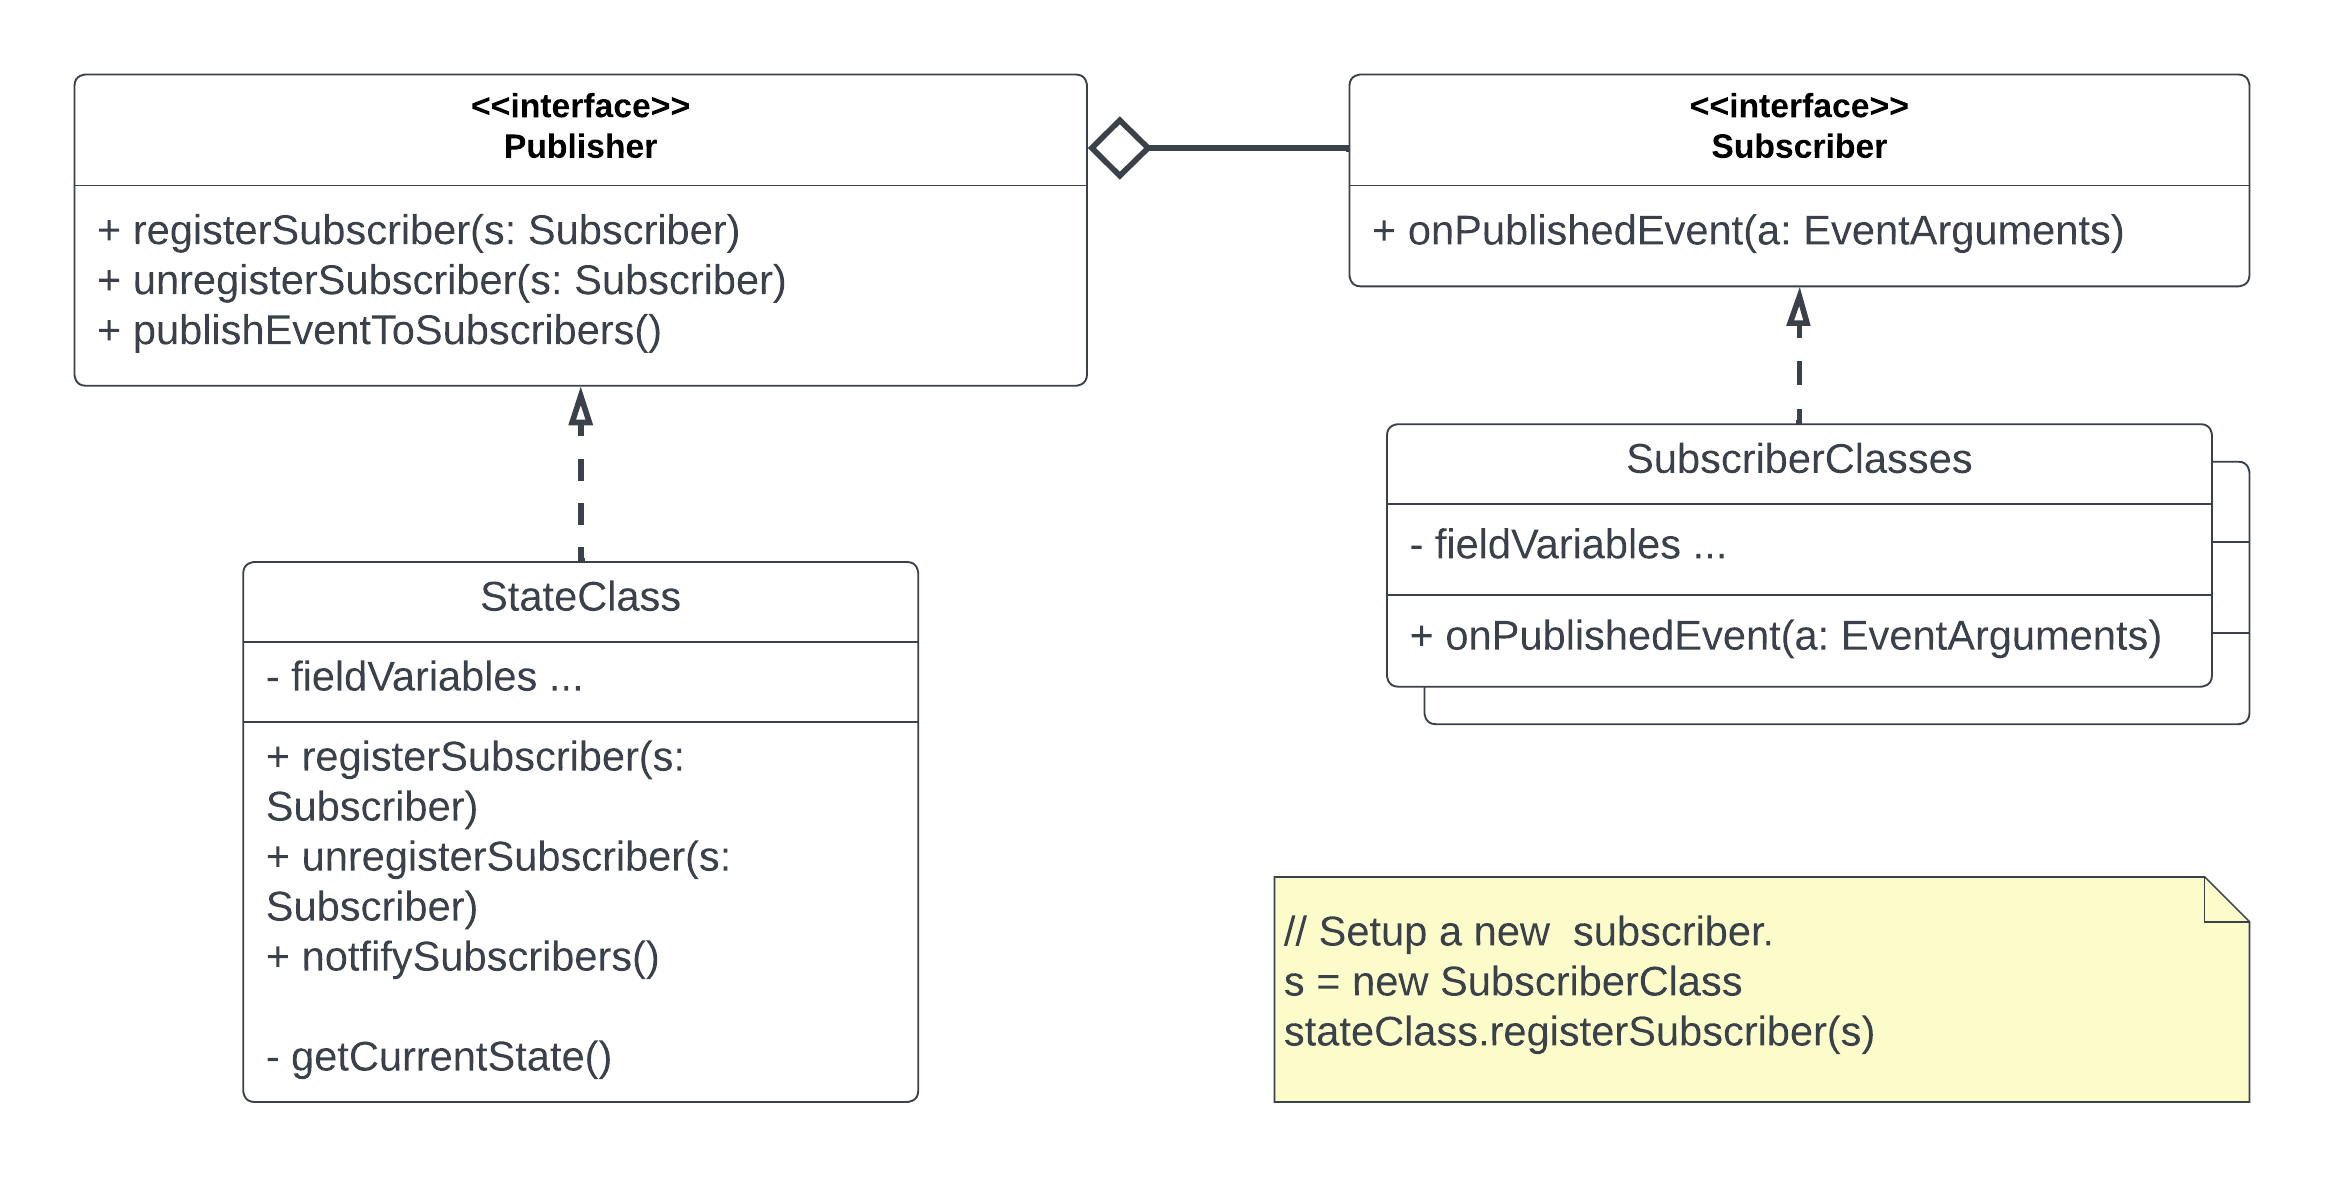
\includegraphics[scale=0.75]{Project_report/figures/theory/design_patterns/observer_uml.png}
      \caption{UML diagram of generic publisher/subscriber-relation implementation.}
      \label{fig:observer_uml}
    \end{figure}

\subsection{Overview of the Observer Pattern in Unity and C\#}
    Both the C\# programming language and the Unity API includes several features that facilitates the use of the Observer pattern. Most modern languages opt for a method-based implementation of the Observer Pattern, as compared to the class-based implementation as seen in Figure \ref{fig:observer_uml}. The list that follows highlights some of the most prominent components that are used to promote the usage of this pattern:

\begin{itemize}
    \item \textbf{Delegates (C\#)}: Define a type representing a specific user-defined method signature, allowing for a method-based event system\cite{microsoft-csharp-delegates}. This custom type can be realized with any method sharing the same signature as the delegate, enabling a type-safe way of passing methods as arguments. They resemble C++ function pointers but provide object-oriented capabilities by encompassing both a function and its associated object instance.
    
    \item \textbf{Event Handlers (C\#)}: Methods defined in the subscriber class that conform to a specific delegate signature\cite{microsoft-eventhandler}, typically a delegate with two parameters: one object representing the publisher and one event data object containing event-specific information. These event handlers are responsible for processing incoming events and performing any necessary actions when the triggering event is published.
    
    \item \textbf{Events (C\#)}: A convenient feature in C\# built upon the foundation of delegates\cite{microsoft-csharp-events}. They provide an easy way to define, subscribe, and publish events in C\#. Publishers define the event, while subscribers can subscribe or unsubscribe using the event handler. Events enforce encapsulation by allowing only the class that owns them to publish them while still enabling other classes to subscribe or unsubscribe at run-time.
    
    \item \textbf{UnityEvents (Unity)}: A built-in event class offering a flexible and powerful way to facilitate event-driven systems that can be configured in a user-friendly way through the Unity editor\cite{unity-unityevents}. Being serializable, they can easily be set up and managed through the editor using a drag-and-drop approach within the editor.
\end{itemize}

\subsection{Singleton}
    The Singleton pattern is a creational pattern that ensures only one instance of a specific class can be created at any given time, providing global access points to that instance. The pattern has garnered criticism for violating core object-oriented principles, such as The Single Responsibility Principle\footnote{The 'S' in SOLID. States that a class should only have one responsibility, promoting good separation of concern and modularity.}, promoting tight coupling, and making testing more difficult due to challenges in isolating tests, replacing instances with mocks, and managing shared global state. However, some argue for its responsible usage, applied only to classes that genuinely require a single instance and where global access is necessary. It is crucial to manage dependencies and shared states carefully to minimize the risk of creating hard-to-maintain, tightly-coupled code. Common use cases for the Singleton pattern in game development include managing access to different manager classes, such as managers for input, audio, or pooling.

    The pattern is implemented by having a private static field in the singleton class for storing the instance of the class. This instance is instantiated through a public static creation method, which uses "lazy initialization" to create a new singleton object instance through a private constructor if it is the first time the instance is being called, or returns the pre-existing instance otherwise. To ensure thread-safety in multi-threaded applications, a locking mechanism can be implemented to prevent multiple threads from creating separate instances simultaneously. This can be achieved using the "double-checked locking" pattern, where the lock is only acquired if the instance is null, reducing the performance overhead of locking in cases when the instance is already created.

\subsection{State}
    The State pattern is a behavioral pattern that creates a modular and extensible system architecture for managing transition between different object states. The pattern does so by decoupling the logic for each possible state into a separate interface. A main class then manages these states by offering methods for interacting with different state objects and delegating any necessary command to the current state when told to. This main class can be described as mediator between different states, and offers the developers an user-friendly way of managing state actions and transitions.

    The pattern was first introduced by the aforementioned book "Design Patterns: Elements of Reusable Object-Oriented Software", and draws its inspiration from the concept of finite state machines (FSM) which are computational model used across a wide spectrum of domains such as control systems and artificial intelligence. A FSM consists of a finite amount of states, the initial state, and the adhering transitions between them. While both FSM and the State pattern deals with managing system behavior through various states and transition, FSM is a more general concept that focuses on the overall structure of a system, while the State pattern is a specific object-oriented concept focusing on adhering to good object-oriented principles.

    By seperating the state logic into a seperate interface, this makes it easy to accommodate for change and extensibility when modifying or adding a new state. This adheres to the Open/Closed principle\footnote{The 'O' in SOLID. Says that a class should be easy to extend without needing to modify any existing code.} as it allows developers to introduce new states without altering the existing state classes or the main class responsible for managing state transitions.

    The pattern is implemented by defining the common State interface, that should be able to handle any state specific requests and transitions. This interface is then realized by concrete states classes that provides their own unique logic and behaviour. To mediate between these states, you then implement a main class, sometimes called the Context class, that holds a reference to the current state and delegates function calls to it. This main class is also responsible for changing the current state based on transition logic defined in the concrete State classes.
    
    \begin{figure}[H]
      \centering
      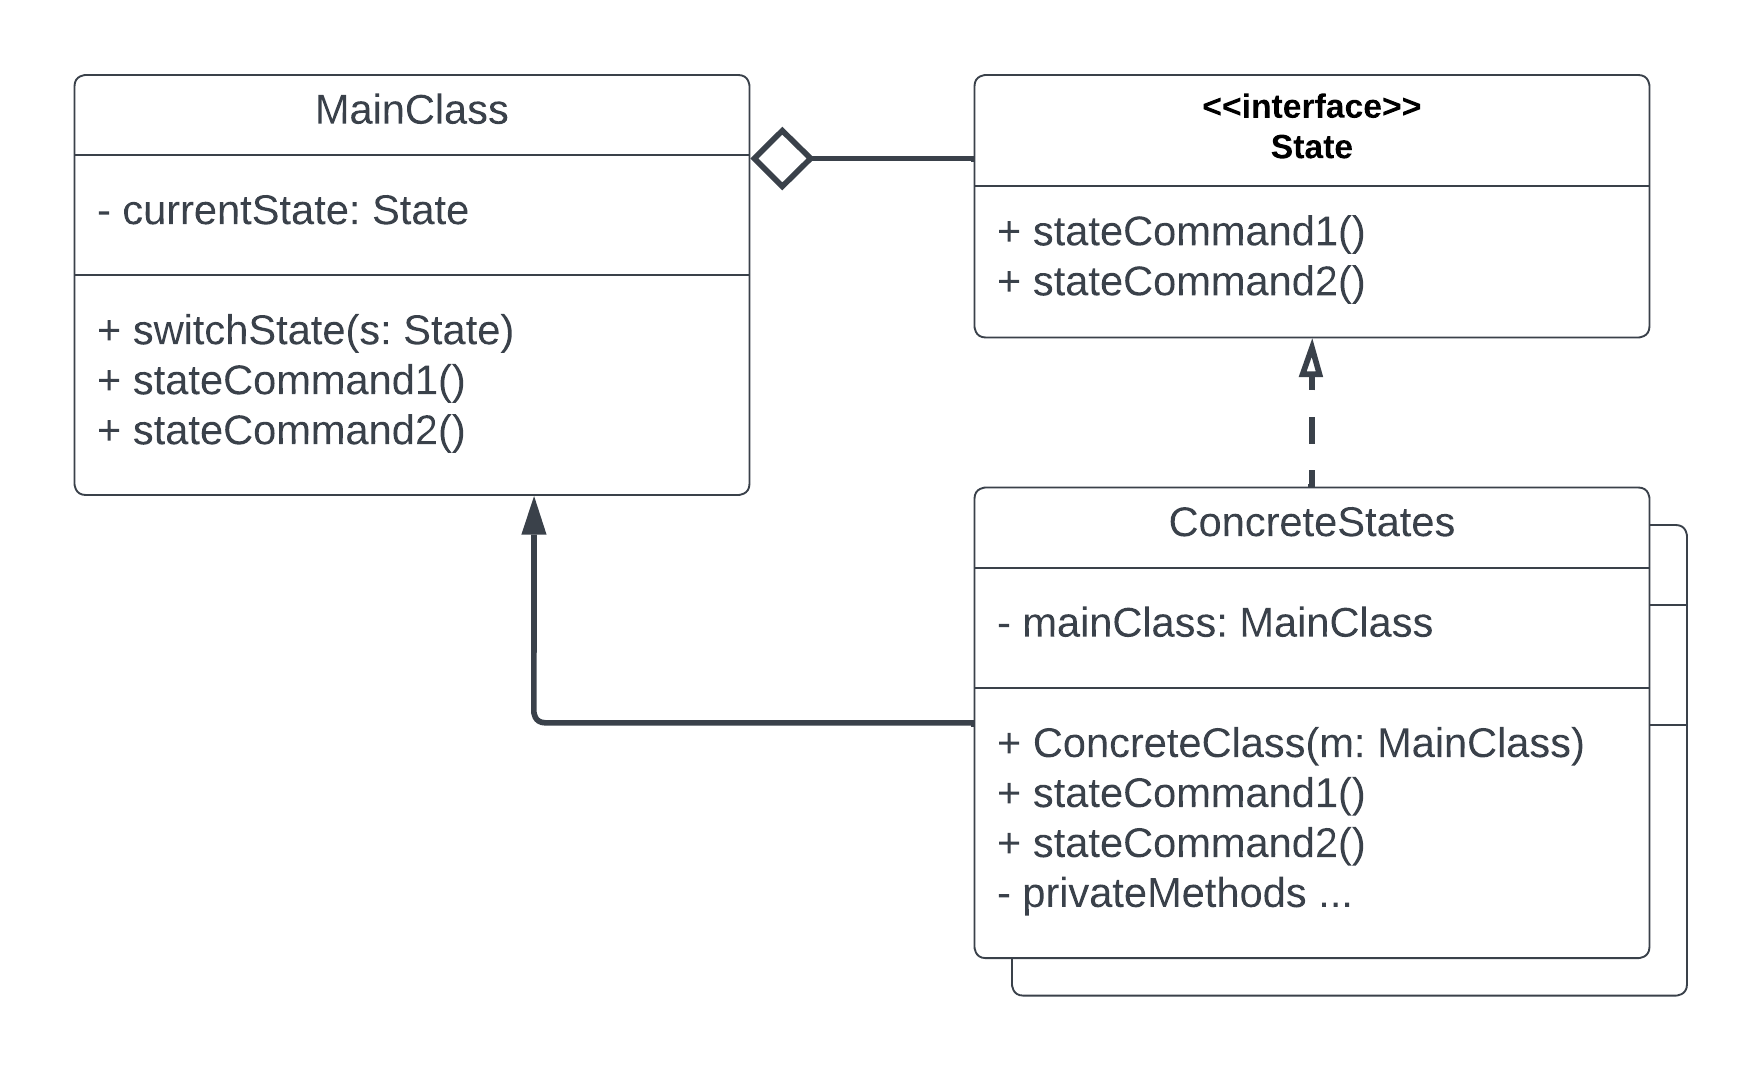
\includegraphics[scale=0.75]{Project_report/figures/theory/design_patterns/state_uml.png}
      \caption{UML diagram of generic State pattern implementation.}
      \label{fig:observer_uml}
    \end{figure}

    \vspace{50pt}
    \begin{itemize}
        \item https://www.amazon.com/-/dp/0195019199
        \item Design Patterns: Elements of Reusable Object-Oriented Software
        \item https://gameprogrammingpatterns.com/observer.html
    \end{itemize}


